%%%%%%%%%%%%
% $Beschreibung: Kurzfassung des Handbuchs für einen schnellen Einstieg 
% $Autor: Hannah Mey $
% $Datum: 10.06.2025 $
% $Pfad: Demonstrator_Schrittmotor\Schnelleinstieg\Schnelleinstieg_Schrittmotor.tex $
% $Version: 1 $
%
%%%%%%%%%%%%
\documentclass[12pt,a4paper]{scrbook}
\usepackage{tikz}
\usepackage{hyperref}

\begin{document}


	
	\chapter{Schnelleinstieg für den Schrittmotor Demonstrator}
	
	\section{Lieferumfang}
	
	\begin{itemize}
		\item Schrittmotor Demonstrator
		\item Netzkabel
	\end{itemize}
	
	\section{Gerät aufstellen}
	\begin{itemize}
		\item Stellen Sie den Schrittmotor Demonstrator auf eine ebene, feste Oberfläche.
		\item Vermeiden Sie direkte Sonneneinstrahlung sowie Wärme- oder Feuchtigkeitsquellen.
		\item Keine Gegenstände auf den Schrittmotor Demonstrator stellen.
		\item Halten Sie den Arbeitsbereich des Schrittmotor Demonstrators frei von Gegenständen.
	\end{itemize}
	
	\section{Inbetriebnahme}
	
	\begin{figure}[htpb]
		\centering
		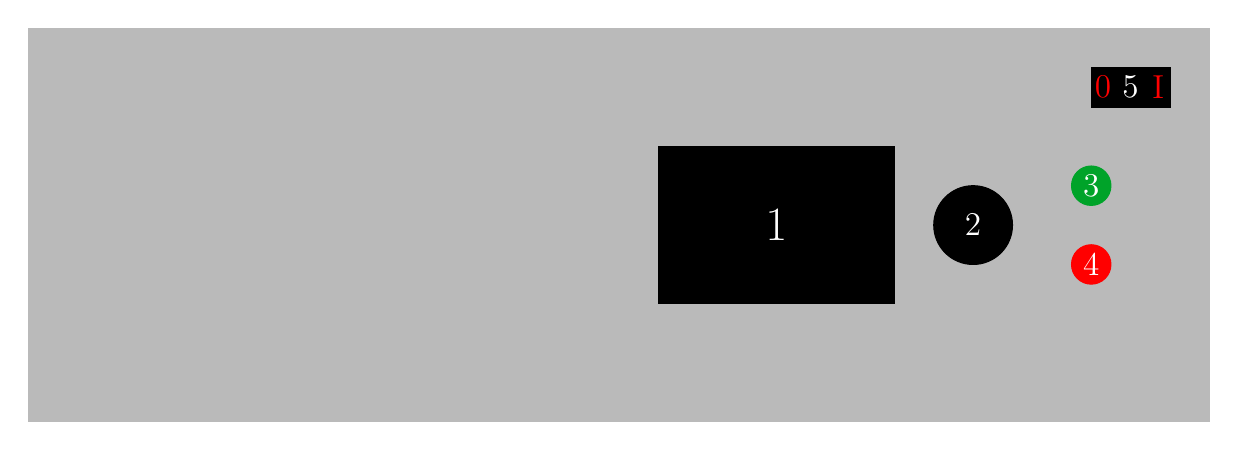
\begin{tikzpicture}
			\tikzstyle{every node}=[font=\LARGE]
		\draw [ color={rgb,255:red,186; green,186; blue,186} , fill={rgb,255:red,186; green,186; blue,186}] (0,5) rectangle (15,0);
		\draw [ fill={rgb,255:red,0; green,0; blue,0} ] (8,3.5) rectangle  node {\Large Display} (11,1.5);
		\draw [ fill={rgb,255:red,0; green,0; blue,0} ] (13.5,4.5) rectangle (14.5,4);
		\node [font=\large, color={rgb,255:red,255; green,0; blue,0}] at (13.65,4.25) {0};
		\node [font=\large, color={rgb,255:red,255; green,0; blue,0}] at (14.35,4.25) {I};
		\draw [ fill={rgb,255:red,0; green,0; blue,0} ] (12,2.5) circle (0.5cm);
		\draw [ color={rgb,255:red,255; green,0; blue,0} , fill={rgb,255:red,255; green,0; blue,0}] (13.5,2) circle (0.25cm);
		\draw [ color={rgb,255:red,0; green,163; blue,41} , fill={rgb,255:red,0; green,163; blue,41}] (13.5,3) circle (0.25cm);
		\node [font=\LARGE, color={rgb,255:red,255; green,255; blue,255}] at (9.5,2.5) {1};
		\node [font=\large, color={rgb,255:red,255; green,255; blue,255}] at (12,2.5) {2};
		\node [font=\large, color={rgb,255:red,255; green,255; blue,255}] at (13.5,3) {3};
		\node [font=\large, color={rgb,255:red,255; green,255; blue,255}] at (13.5,2) {4};
		\node [font=\large, color={rgb,255:red,255; green,255; blue,255}] at (14,4.25) {5};
		\end{tikzpicture}
		\caption{Elemente auf der Frontblende des Demonstrators}
		\label{tikz:Frontblende}
	\end{figure}
	
	\begin{enumerate}
		\item \textbf{Stromversorgung:}
		\begin{itemize}
			\item Stecken Sie den Stecker des Netzkabels in die Steckdose.
		\end{itemize}
		\item \textbf{Einschalten:}
		\begin{itemize}
			\item Gerät über Ein/Ausschalter (Figure \ref{tikz:Frontblende}: 5) einschalten.
			\item Bitte warten, bis OLED-Display (Figure \ref{tikz:Frontblende}: 1) "SYSTEM AKTIV; Willkommen!; Stufe waehlen" anzeigt, dann ist das System bereit.
		\end{itemize}
		\item \textbf{Bewegungsstufe auswählen:}
		\begin{itemize}
			\item Dreh-Encoder (Figure \ref{tikz:Frontblende}: 2) drehen, um Bewegungsstufe auszuwählen.
			\item Geschwindigkeiten der Bewegungsstufen sind Tabelle \ref{tab:Bewegungsstufen} zu entnehmen und werden auf dem OLED-Display angezeigt.
		\end{itemize}
		\item \textbf{Starten:}
		\begin{itemize}
			\item Der Bewegungsablauf wird über den grünen Start-Knopf (Figure \ref{tikz:Frontblende}: 3) gestartet.
		\end{itemize}
		\item \textbf{Stoppen:}
		\begin{itemize}
			\item Der Bewegungsablauf stoppt automatisch, wenn der Motor in den Endschalter fährt. Nach Ende des Bewegungsablaufs, kann die gemessene Geschwindigkeit des Geschwindigkeitssensors auf dem OLED-Display abgelesen werden. 
			\item Wenn der Bewegungsablauf durch einen Notfall unterbrochen werden muss, dann betätigen Sie den roten Stopp-Knopf (Figure \ref{tikz:Frontblende}: 4).
		\end{itemize}
	\end{enumerate}
	
		\section{Bewegungsstufen}
		
		\begin{table}[htpb]
			\centering
			\begin{tabular}{|c|c|}
				\hline
				\textbf{Bewegungsstufe} & \textbf{Geschwindigkeit in cm/s} \\
				\hline
				1 & 1,33 \\
				2 & 2,00 \\
				3 & 2,22 \\
				4 & 2,50 \\
				5 & 3,33 \\
				\hline
			\end{tabular}
			\caption{Bewegungsstufen}
			\label{tab:Bewegungsstufen}
		\end{table}
	


		
\end{document}